%% LyX 2.0.2 created this file.  For more info, see http://www.lyx.org/.
%% Do not edit unless you really know what you are doing.
\documentclass[onecolumn,english]{IEEEtran}
\usepackage[T1]{fontenc}
\usepackage{babel}
\usepackage{graphicx}
\usepackage[unicode=true,
 bookmarks=true,bookmarksnumbered=true,bookmarksopen=true,bookmarksopenlevel=1,
 breaklinks=false,pdfborder={0 0 0},backref=false,colorlinks=false]
 {hyperref}
\hypersetup{pdftitle={Your Title},
 pdfauthor={Your Name},
 pdfpagelayout=OneColumn, pdfnewwindow=true, pdfstartview=XYZ, plainpages=false}

\makeatletter

%%%%%%%%%%%%%%%%%%%%%%%%%%%%%% LyX specific LaTeX commands.
%% Because html converters don't know tabularnewline
\providecommand{\tabularnewline}{\\}

%%%%%%%%%%%%%%%%%%%%%%%%%%%%%% Textclass specific LaTeX commands.
 % protect \markboth against an old bug reintroduced in babel >= 3.8g
 \let\oldforeign@language\foreign@language
 \DeclareRobustCommand{\foreign@language}[1]{%
   \lowercase{\oldforeign@language{#1}}}

%%%%%%%%%%%%%%%%%%%%%%%%%%%%%% User specified LaTeX commands.
% for subfigures/subtables
\ifCLASSOPTIONcompsoc
\usepackage[caption=false,font=normalsize,labelfont=sf,textfont=sf]{subfig}
\else
\usepackage[caption=false,font=footnotesize]{subfig}
\fi

\makeatother

\begin{document}





\title{Peak2Cloud: Scientific Computing in the Cloud}


\author{Joseph Anthony C.~Hermocilla %
\thanks{E-mail: \protect\href{mailto:jchermocilla@up.edu.ph}{jchermocilla@up.edu.ph}.%
}}


\markboth{ICS Technical Reports, Vol. 2014, No. 1, January-June 2014}{Joseph
Anthony Hermocilla : Peak2Cloud: Scientific Computing in the Cloud}


\IEEEpubid{\copyright~2014 Institute of Computer Science, University of the
Philippines Los Banos}
\maketitle
\begin{abstract}
Peak2Cloud (P2C) is an Openstack-based private cloud deployed as testbed
for scientific computing. We present how P2C was setup, configured,
and tested. We also describe vcluster, a tool for rapidly deploying
message-passing clusters on P2C. Lastly, we present an analysis of
some benchmark results on the performance of P2C deployed virtual
clusters.\end{abstract}
\begin{IEEEkeywords}
cloud computing, scientific computing, high-performance computing,
message passing
\end{IEEEkeywords}

\section{Introduction}

\IEEEPARstart{ C}{loud} computing has become a buzzword in today's
modern computing, though there is no agreed upon meaning of the term.
In 2011, NIST \cite{mell_nist_2011} published a definition that is
widely quoted and used. The popularity of cloud computing mainly comes
from its ability to provision additional resources on demand with
minimum intervention from the provider. It leverages advances in virtualization
and web services technologies. For example, a website with a sudden
increase in workload can start another server machine (virtual) almost
instantaneously to accommodate the additional load.

Cloud computing offers service models which include Software-as-a-Service(SaaS),
Platform-as-a-Service(PaaS), and Infrastructure-as-a-Service(IaaS).
IaaS allows the consumer to provision computing resources(hardware,
network, storage) to run arbitrary software including operating systems
\cite{mell_nist_2011}. 


\section{Related Work}

Studies have been published to evaluate the applicability of the cloud
for scientific computing.\cite{ekanayake_high_2010} \cite{evangelinos_cloud_2008}\cite{exposito_performance_2013}\cite{ludescher_cloud-based_2013}\cite{mauch_high_2013}\cite{jackson_performance_2010}\cite{zhai_cloud_2011}\cite{walker_benchmarking_????}.Most
of these utilized the public cloud, specifically Amazon EC2 as their
testbed.


\subsection{subsection}


\subsection{another subsection}


\section{Methodology}


\subsection{Openstack}


\subsection{Hardware Requirements}


\subsection{Network Architecture}


\subsection{vcluster}


\subsection{Benchmarks}


\section{Results and Discussion}

\begin{figure}[htbp]
\begin{centering}
\textsf{A single column figure goes here}
\par\end{centering}

\caption{Captions go \emph{under} the figure}
\end{figure}
\begin{table}[htbp]
\caption{Table captions go \emph{above} the table}


\centering{}%
\begin{tabular}{|c|c|}
\hline 
delete & this\tabularnewline
\hline 
\hline 
example & table\tabularnewline
\hline 
\end{tabular}
\end{table}



\section{Conclusions}

bla bla


\appendices{}


\section{First appendix}

Citation: 


\section{Second appendix}


\section*{Acknowlegment}

This work is funded through the Department of Science and Technology
(DOST) Accelerated Science and Technology Human Resource Development
Program (ASTHRD) scholarship.

\bibliographystyle{IEEEtran}
\bibliography{p2cpaper}

\begin{IEEEbiography}[{{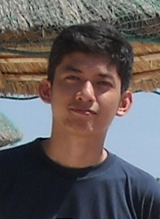
\includegraphics[clip,width=1in,height=1.25in]{me-new}}}]
{Joseph Anthony C. Hermocilla} obtained his MS in Computer Science
from the University of the Philippines Los Banos where he is currently
an assistant professor at the Institute of Computer Science and head
of the Systems Research Group. His research interests span the area
of systems, including operating systems, computer architecture, data
communications and networking, distributed systems, computer security,
and high-performance computing. He is a member of the Computing Society
of the Philippines and the Philippine Society of Information Technology
Educators.
\end{IEEEbiography}

\end{document}
